\documentclass{article}
\usepackage[utf8]{inputenc}
\usepackage[T2A]{fontenc}
\usepackage[russian]{babel}
\usepackage{graphicx}
\usepackage{float}

\title{Отчет OS Лаб-5}
\author{Гаврилюк Виталий М3232}
\date{}

\begin{document}

\maketitle

\begin{itemize}
\item Общий размер оперативной памяти: 858Mi 
\item Объём раздела подкачки: 859Mi 
\item Размер страницы виртуальной памяти: 4кб 
\item Объем свободной физической памяти в ненагруженной системе: 692Mi 
\item Объем свободного пространства в разделе подкачки в ненагруженной системе: 768Mi 
\end{itemize}

\section*{Эксперимент 1}

\subsection*{Первый этап} 

\begin{figure}[H]
\centering
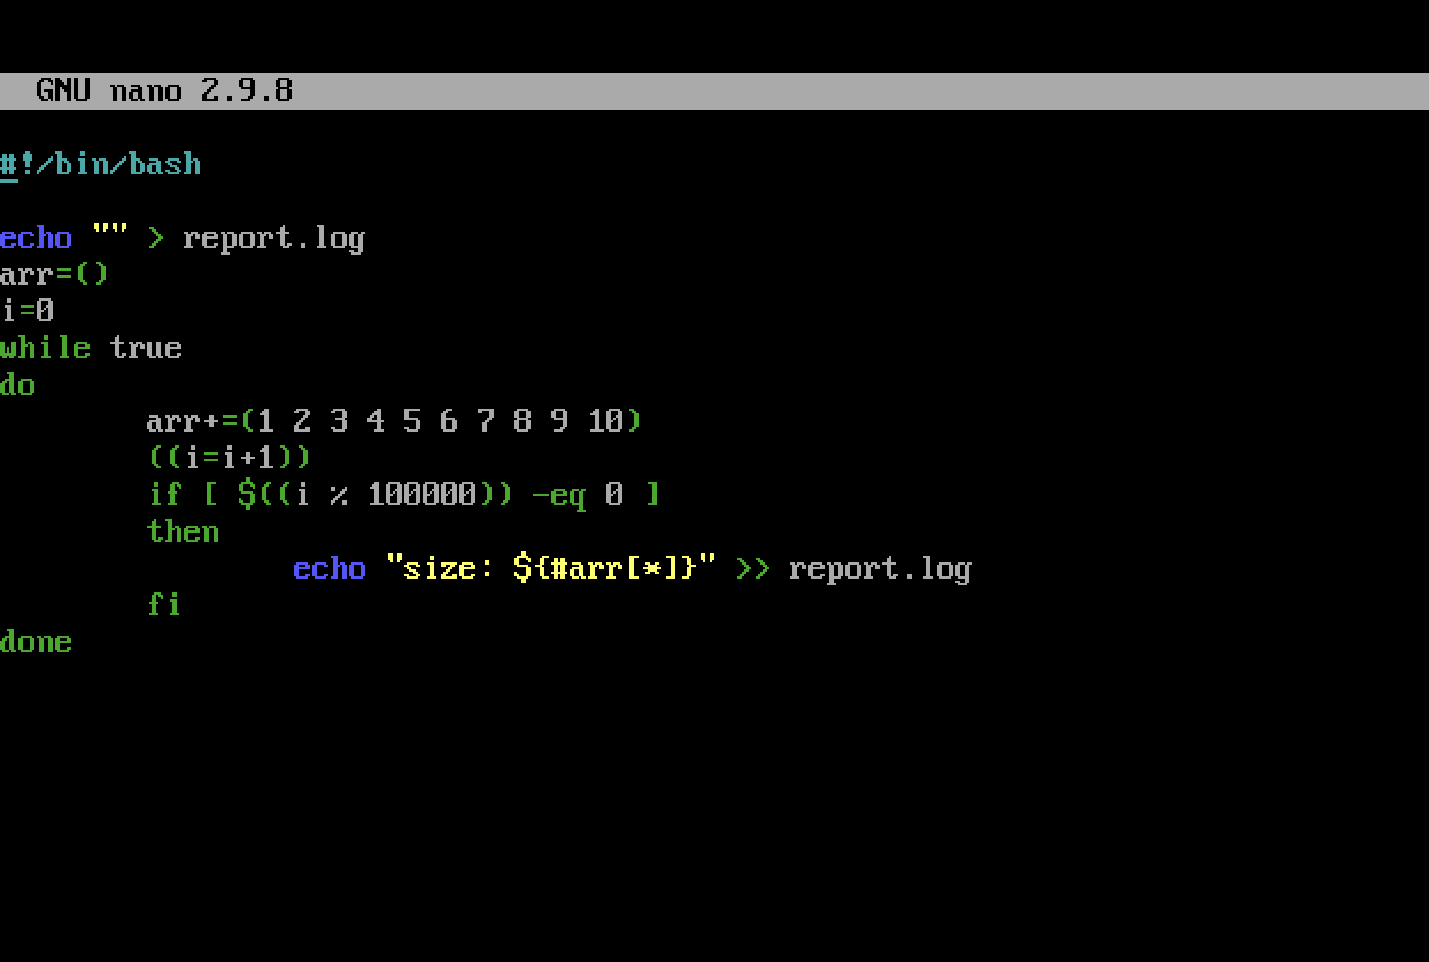
\includegraphics[width=0.8\textwidth]{images/1.png}
\caption{Mem.bash}
\end{figure} 

\begin{figure}[H]
\centering
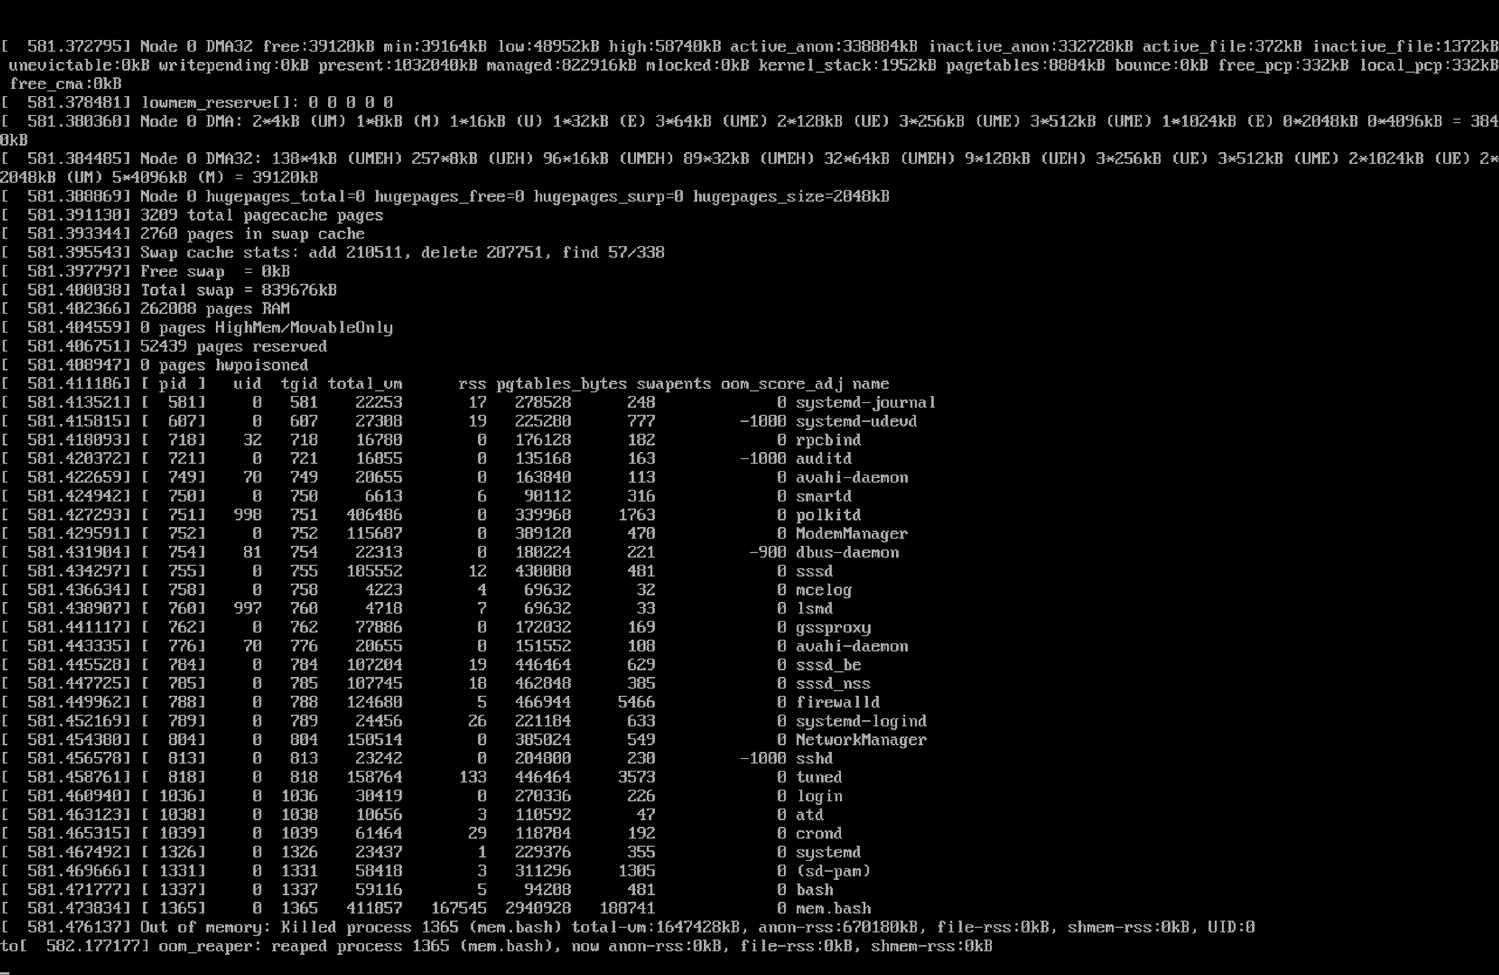
\includegraphics[width=0.8\textwidth]{images/2.png}
\caption{Сообщение о падении}
\end{figure}

Последний размер массива: 18 000 000 

\begin{figure}[H]
\centering
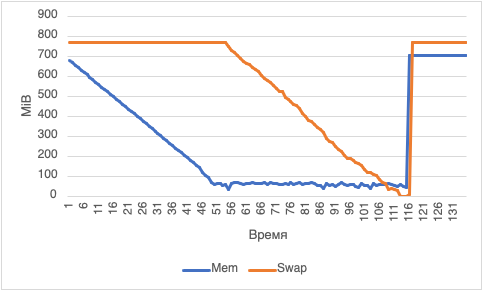
\includegraphics[width=0.8\textwidth]{images/3.png}
\caption{}
\end{figure}

\begin{figure}[H]
\centering
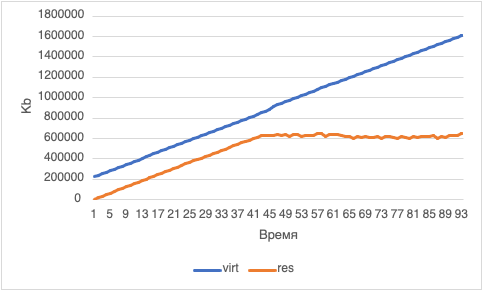
\includegraphics[width=0.8\textwidth]{images/4.png}
\caption{}
\end{figure}

Вывод: сначала заполняется оперативная память. Когда она заканчивается, используется файл подкачки. Если и тут память закончилась, система вынуждена убить процесс. 

\subsection*{Второй этап}

\begin{figure}[H]
\centering
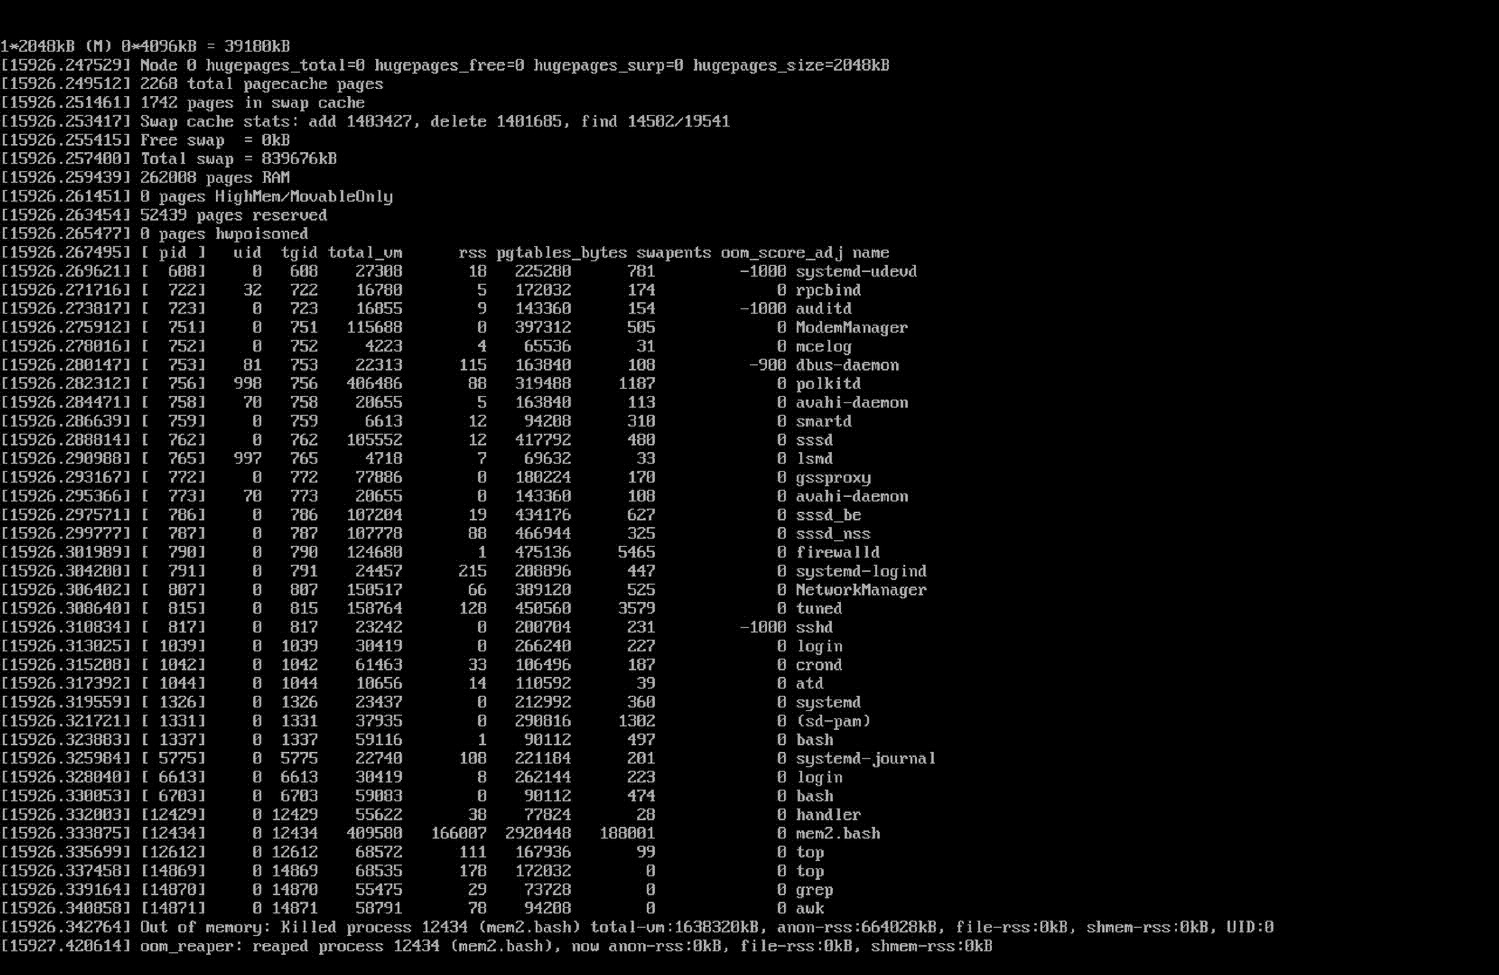
\includegraphics[width=0.8\textwidth]{images/5.png}
\caption{Падение второго скрипта}
\end{figure}

\begin{figure}[H]
\centering
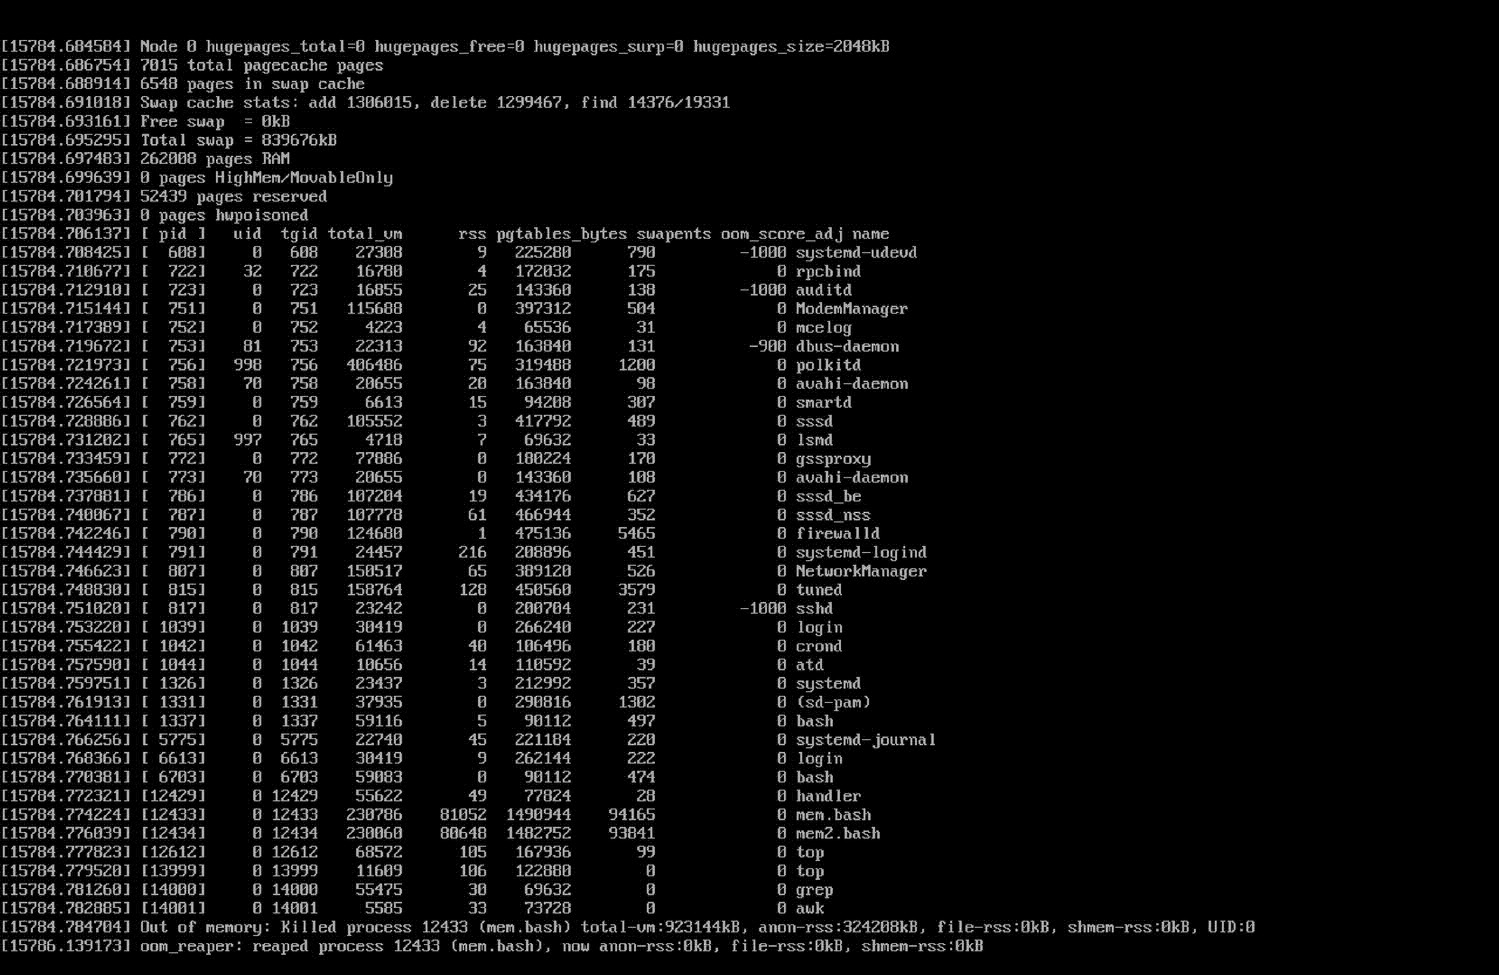
\includegraphics[width=0.8\textwidth]{images/6.png}
\caption{Падение первого скрипта}
\end{figure}

\hspace{4mm}
Report1 size: 8 000 000 

Report2 size: 16 000 000

\begin{figure}[H]
\centering
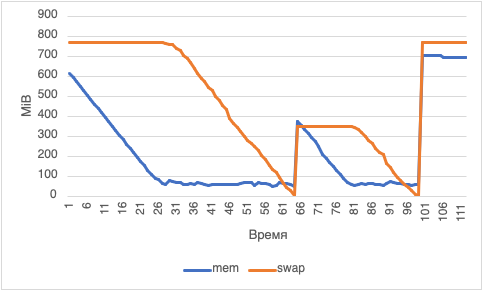
\includegraphics[width=0.8\textwidth]{images/7.png}
\caption{}
\end{figure}

\begin{figure}[H]
\centering
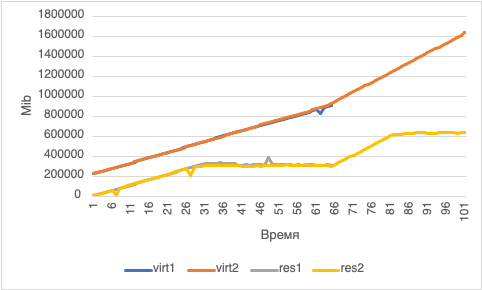
\includegraphics[width=0.8\textwidth]{images/8.png}
\caption{}
\end{figure}

Вывод: сначала заполняется оперативная память. Когда она заканчивается, используется файл подкачки. Если и тут память закончилась, система вынуждена убить процесс. Как только она его убивает, освобождается используемая им память. После того, как память снова заканчивается, система убивает второй процесс. 

\section*{Эксперимент 2}

Первый этап. 

\begin{figure}[H]
\centering
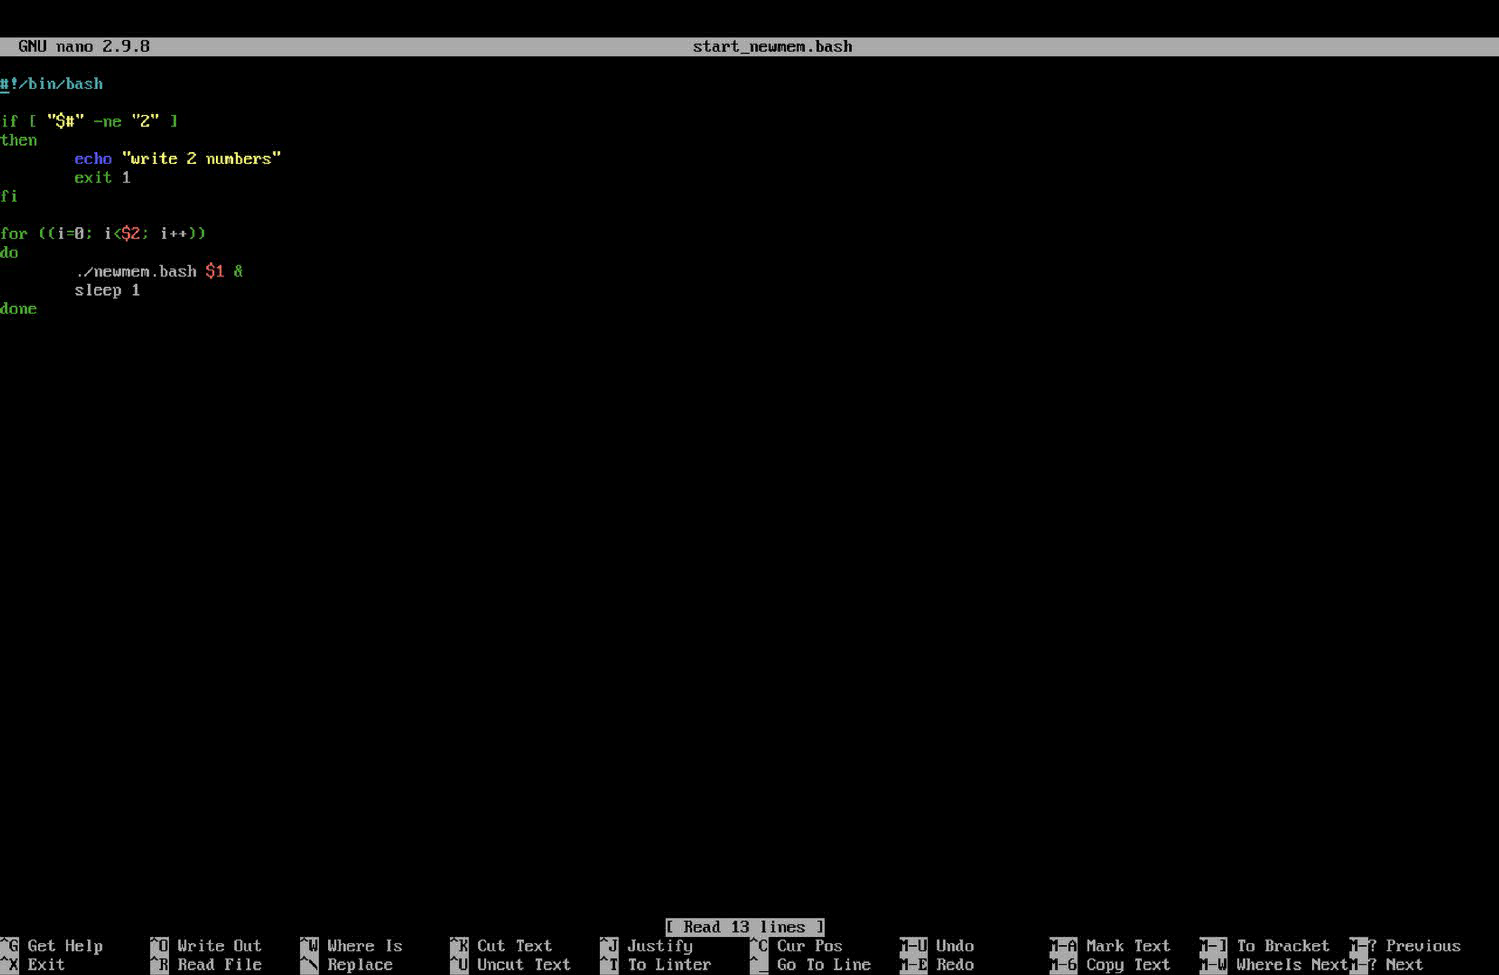
\includegraphics[width=0.8\textwidth]{images/9.png}
\caption{newmem.bash}
\end{figure}

\begin{figure}[H]
\centering
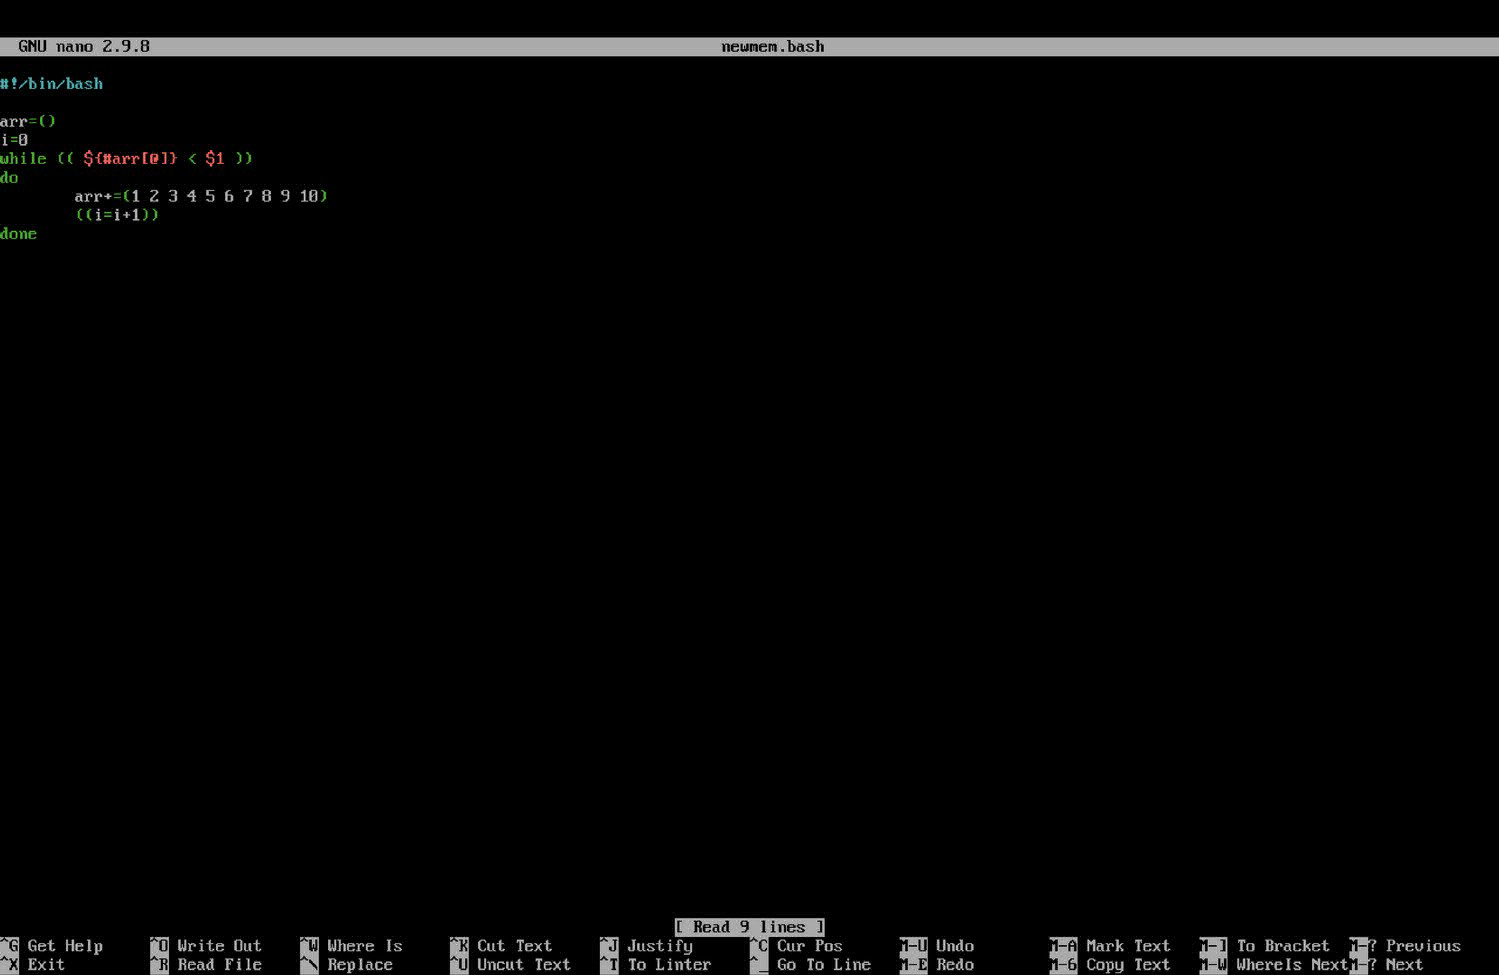
\includegraphics[width=0.8\textwidth]{images/10.png}
\caption{start-newmem.bash}
\end{figure}

Я взял N = 1 600 000, К = 10. Все скрипты успешно завершили свою работу.\\  

При К = 30, N = 1 600 000 ряд процессов закончился аварийно, т.к. процессы требуют суммарно приблизительно в 3 раза больше оперативной памяти, чем доступно. \\

Максимальное значение N, такое что при К = 30 не происходило бы аварийных остановок процессов равно $9 * 10^7$. Оно отличается от ожидаемого значения $2.38 * 10^9 / 30$, что примерно равно $8 * 10^7$, т.к. процессы не работают синхронно и некоторые достигают штатного завершения раньше других, пока оперативной памяти хватает. 

\end{document}